\documentclass[11pt,openany]{book}
\usepackage[a4paper,margin=1in]{geometry}
\usepackage{macros}

\title{Protoespacio Dirac--Weyl:\\
de grafeno y caminatas discretas\\
a la ecuacion de Dirac en \texorpdfstring{$3+1$}{(3+1)}}
\author{Nelson Bolivar}
\date{\today}

\begin{document}
\frontmatter
\maketitle
\tableofcontents

\chapter*{Prefacio}
\addcontentsline{toc}{chapter}{Prefacio}

Este libro consolida la serie de borradores fechados en marzo y abril de 2026
sobre la emergencia de la ecuacion de Dirac en $3+1$ desde dinamicas
discretas. Su politica editorial es estricta: cada afirmacion algebraica o
combinatoria significativa esta acompanada por una verificacion automatica
(\texttt{sympy} para algebra simbolica, \texttt{z3} para satisfacibilidad
logica), ejecutada antes de cada compilacion del manuscrito.

Cuando un lema indica
\begin{quote}\small\texttt{\% verified-by: validators/<modulo>.py::<test>}\end{quote}
significa que el test correspondiente debe pasar bajo el \texttt{pytest} del
repositorio para que el PDF pueda generarse.

\chapter{Introduccion}

\section{Pregunta motora}

La pregunta de fondo de esta investigacion es si la estructura covariante
relativista en $3+1$ dimensiones --- algebra de Clifford, generadores de
Lorentz, $SL(2,\mathbb{C})$, fermiones de Dirac y Weyl --- puede entenderse
como un \emph{sector efectivo infrarrojo} de un sustrato discreto local mas
fundamental, al que llamamos \emph{protoespacio}.

\section{Hipotesis de trabajo}

\begin{enumerate}[label=(H\arabic*)]
  \item \textbf{Emergencia infrarroja:} el continuo relativista no describe el
        objeto microscopico exacto, sino solo su sector de baja energia y
        longitudes de onda grandes.
  \item \textbf{Primacia de la localidad:} la propiedad robusta de partida es
        la localidad del paso unitario \Uop. La covariancia Lorentz aparece
        despues, si aparece.
  \item \textbf{Sustrato ampliado:} el protoespacio no es la red espacial
        desnuda, sino la tupla
        \[\Proto \sim \ProtoTuple.\]
\end{enumerate}

\section{Plan del libro}

La Parte~I construye la escalera $1D \to 2D \to 3D \to 3+1$ a traves de SSH,
grafeno, semimetales de Weyl/Dirac y caminatas cuanticas. La Parte~II extrae
la estructura espinorial y los generadores de Lorentz como objetos
emergentes. La Parte~III enuncia criterios para que un sistema discreto
admita un cono de luz, isotropia e invariancia Lorentz efectivos. La
Parte~IV deja abiertos los dos nudos identificados en la revision del 28 de
marzo: el espectro global tipo Brillouin del paso discreto, y la
formulacion del protoespacio independiente del lenguaje reciproco.

\chapter{Notacion y supuestos comunes}
\label{ch:notacion}

\section{Variables de momento}

\begin{align}
\vk &:\ \text{momento de Bloch o variable global del espacio reciproco},\\
\vq &:\ \text{desviacion pequena respecto de un nodo o punto de expansion},\\
\vp &:\ \text{momento efectivo continuo en el sector infrarrojo}.
\end{align}

Regla practica:
\begin{enumerate}[label=\arabic*.]
  \item \vk\ cuando hablemos del modelo discreto exacto;
  \item $\vk = \vk_0 + \vq$ al linealizar alrededor de un nodo;
  \item \vp\ una vez pasado al lenguaje efectivo continuo.
\end{enumerate}

\section{Espacios internos}

\begin{align}
\sigma_i &:\ \text{grado de libertad tipo Weyl / pseudospin de dos componentes},\\
\tau_i   &:\ \text{indice quiral o bloque Weyl acoplado}.
\end{align}

La forma canonica del bloque Dirac efectivo queda:
\begin{equation}
\HD = v\,\tau_z\otimes(\sigma_x p_x + \sigma_y p_y + \sigma_z p_z)
      + m\,\tau_x \otimes \bbI .
\label{eq:HDcanon}
\end{equation}

\section{Objetos dinamicos}

\(\Hop\) denota un Hamiltoniano efectivo o continuo; \(\Uop\) denota el paso
unitario discreto exacto. En particular \UW\ es la caminata Weyl minima y
\UD\ la caminata Dirac de cuatro componentes.

\section{Tres niveles}

\begin{description}
  \item[\NivelI] red discreta, localidad de \Uop, grupo de simetrias
        discretas exactas, periodicidad de cuasienergia.
  \item[\NivelII] linealizacion en un nodo, bloques Weyl/Dirac, isotropia
        aproximada, masa y velocidad efectivas.
  \item[\NivelIII] \gmu, algebra de Clifford, generadores de Lorentz,
        $SO^+(3,1)$, Poincare, $SL(2,\mathbb{C})$ como \emph{organizacion
        del limite efectivo}.
\end{description}

\section{Convenciones de lenguaje}

\begin{itemize}[leftmargin=*]
  \item \enquote{exacto}: simetrias de \Uop\ para todo \vk; identidades
        algebraicas cerradas; resultados independientes de expansion en \vq.
  \item \enquote{efectivo}: Hamiltonianos linealizados; isotropia emergente;
        Lorentz/Poincare como simetrias del limite continuo.
  \item \enquote{protoespacio}: la tupla \Proto, nunca una sola de sus
        proyecciones.
\end{itemize}


\mainmatter
% --- Parte I: ruta 1D -> 2D -> 3D -> 3+1
\part{De la red discreta a Dirac efectivo}
% % Importado desde: 2026-03-28_SSH_a_Dirac_1D.tex
\chapter{Derivacion Pedagogica: --- Del modelo SSH a una ecuacion de Dirac en \(1+1\)}
\label{ch:ssh-a-dirac-1d}






% verified-by: validators/ssh.py::test_ssh_squared
% verified-by: validators/ssh.py::test_ssh_gap_closes
% verified-by: validators/ssh.py::test_ssh_linearization

\section{Objetivo}

El modelo de Su--Schrieffer--Heeger (SSH) es el ejemplo unidimensional correcto para introducir una estructura espinorial efectiva en una red discreta. Su importancia dentro del programa de investigación es muy concreta:

\begin{enumerate}[leftmargin=*]
  \item tiene dos sitios por celda unitaria;
  \item el Hamiltoniano vive naturalmente en un espacio de dos componentes;
  \item el cierre del gap se controla con un parámetro;
  \item al linealizar cerca del punto crítico aparece un Hamiltoniano tipo Dirac en \(1+1\).
\end{enumerate}

En este documento vamos a derivar eso paso a paso, con cuentas intermedias y figuras, para dejar fijo el primer peldaño de la escalera conceptual del proyecto.

\section{La idea física del modelo SSH}

El modelo describe una cadena unidimensional con dos sitios por celda unitaria, que llamaremos \(A\) y \(B\). Los acoplos entre vecinos alternan entre dos valores:
\begin{equation}
t_1 \quad \text{e} \quad t_2.
\end{equation}

Esa alternancia es exactamente lo que permite abrir o cerrar un gap. Cuando \(t_1\neq t_2\), el sistema está gapped. Cuando \(t_1=t_2\), las bandas se tocan en el borde de la zona de Brillouin, y la teoría efectiva se vuelve de tipo Dirac.

\begin{figure}[ht]
\centering
\begin{tikzpicture}[>=Latex,scale=1.2]
  \foreach \x in {0,2,4,6}
    \fill[blue!70] (\x,0) circle (2.2pt);
  \foreach \x in {1,3,5,7}
    \fill[orange!85!black] (\x,0) circle (2.2pt);

  \foreach \x/\lab in {0/A_n,2/A_{n+1},4/A_{n+2}}
    \node[above] at (\x,0) {\small $\lab$};
  \foreach \x/\lab in {1/B_n,3/B_{n+1},5/B_{n+2}}
    \node[above] at (\x,0) {\small $\lab$};

  \draw[very thick] (0,0)--(1,0);
  \draw[very thick,dashed] (1,0)--(2,0);
  \draw[very thick] (2,0)--(3,0);
  \draw[very thick,dashed] (3,0)--(4,0);
  \draw[very thick] (4,0)--(5,0);
  \draw[very thick,dashed] (5,0)--(6,0);
  \draw[very thick] (6,0)--(7,0);

  \node[below] at (0.5,0) {$t_1$};
  \node[below] at (1.5,0) {$t_2$};
  \node[below] at (2.5,0) {$t_1$};
  \node[below] at (3.5,0) {$t_2$};
  \node[below] at (4.5,0) {$t_1$};
  \node[below] at (5.5,0) {$t_2$};

  \draw[decorate,decoration={brace,amplitude=5pt}] (-0.05,-0.55) -- (1.05,-0.55);
  \node[below=7pt] at (0.5,-0.55) {\small celda \(n\)};
  \draw[decorate,decoration={brace,amplitude=5pt}] (1.95,-0.55) -- (3.05,-0.55);
  \node[below=7pt] at (2.5,-0.55) {\small celda \(n+1\)};
\end{tikzpicture}
\caption{Cadena SSH. Cada celda unitaria contiene dos sitios, \(A\) y \(B\). El acoplo intracelda es \(t_1\) y el acoplo interceldas es \(t_2\).}
\label{c01:fig:ssh-chain}
\end{figure}

\section{Hamiltoniano tight-binding}

\subsection{Hamiltoniano en espacio real}

Denotemos por \(a_n^\dagger\) y \(b_n^\dagger\) los operadores de creación en los sitios \(A_n\) y \(B_n\). El Hamiltoniano SSH es
\begin{equation}
H =
\sum_n \left(
t_1\, a_n^\dagger b_n
+ t_2\, a_{n+1}^\dagger b_n
+ \text{h.c.}
\right).
\label{c01:eq:ssh-real}
\end{equation}

Su lectura física es directa:

\begin{enumerate}[leftmargin=*]
  \item \(t_1\) conecta \(A_n\) con \(B_n\) dentro de la misma celda;
  \item \(t_2\) conecta \(B_n\) con \(A_{n+1}\) entre celdas vecinas.
\end{enumerate}

\subsection{Por qué aparecen dos componentes}

Como hay dos sitios por celda unitaria, la función de onda de Bloch debe tener dos componentes:
\begin{equation}
\Psi_k =
\begin{pmatrix}
\psi_A(k)\\
\psi_B(k)
\end{pmatrix}.
\end{equation}

Eso es el análogo unidimensional del pseudospín de subred que luego aparece en grafeno. No es espín real; es el espacio interno \(A/B\) de la cadena.

\section{Paso al espacio recíproco}

\subsection{Transformada de Fourier}

Tomamos
\begin{equation}
a_n=\frac{1}{\sqrt{N}}\sum_k \ee^{\ii k n a} a_k,
\qquad
b_n=\frac{1}{\sqrt{N}}\sum_k \ee^{\ii k n a} b_k,
\label{c01:eq:ssh-fourier}
\end{equation}
donde \(a\) es la longitud de la celda y \(N\) el número de celdas.

Sustituimos \eqref{c01:eq:ssh-fourier} en \eqref{c01:eq:ssh-real}. El término intracelda queda
\begin{equation}
\sum_n t_1 a_n^\dagger b_n
=
t_1 \sum_k a_k^\dagger b_k,
\end{equation}
mientras que el término interceldas produce un factor de fase:
\begin{equation}
\sum_n t_2 a_{n+1}^\dagger b_n
=
t_2 \sum_k \ee^{-\ii k a} a_k^\dagger b_k.
\end{equation}

Por tanto,
\begin{equation}
H=\sum_k
\begin{pmatrix}
a_k^\dagger & b_k^\dagger
\end{pmatrix}
H(k)
\begin{pmatrix}
a_k\\
b_k
\end{pmatrix},
\end{equation}
con
\begin{equation}
H(k)=
\begin{pmatrix}
0 & t_1+t_2\ee^{-\ii k a}\\
t_1+t_2\ee^{\ii k a} & 0
\end{pmatrix}.
\label{c01:eq:ssh-bloch}
\end{equation}

\subsection{Escritura con matrices de Pauli}

Separando partes real e imaginaria,
\begin{equation}
t_1+t_2\ee^{-\ii ka}
=
t_1+t_2\cos(ka)-\ii t_2\sin(ka).
\end{equation}

Entonces el Hamiltoniano se puede escribir como
\begin{equation}
H(k)= d_x(k)\sigma_x + d_y(k)\sigma_y,
\end{equation}
con
\begin{equation}
d_x(k)=t_1+t_2\cos(ka),
\qquad
d_y(k)=t_2\sin(ka).
\label{c01:eq:ssh-dxdy}
\end{equation}

Dependiendo de la convención, el signo delante de \(\sigma_y\) puede cambiar. La física no cambia.

\section{Bandas y cierre del gap}

\subsection{Autovalores}

Como el Hamiltoniano es de la forma \(H=\bm{d}\cdot\bm{\sigma}\), los autovalores son
\begin{equation}
E_\pm(k)=\pm \sqrt{d_x(k)^2+d_y(k)^2}.
\end{equation}

Sustituyendo \eqref{c01:eq:ssh-dxdy},
\begin{equation}
E_\pm(k)=
\pm \sqrt{(t_1+t_2\cos ka)^2+t_2^2\sin^2 ka}.
\end{equation}

Agrupando,
\begin{equation}
E_\pm(k)=
\pm \sqrt{t_1^2+t_2^2+2t_1 t_2 \cos(ka)}.
\label{c01:eq:ssh-dispersion}
\end{equation}

\subsection{Condición de cierre del gap}

Para que las bandas se toquen, debe ocurrir
\begin{equation}
d_x(k)=0,
\qquad
d_y(k)=0.
\end{equation}

La segunda ecuación exige
\begin{equation}
\sin(ka)=0
\quad \Longrightarrow \quad
ka=0,\pi.
\end{equation}

Probamos esos dos casos:

\begin{enumerate}[leftmargin=*]
  \item si \(ka=0\), entonces \(d_x=t_1+t_2\), que no se anula salvo en el caso trivial \(t_1=-t_2\);
  \item si \(ka=\pi\), entonces \(d_x=t_1-t_2\).
\end{enumerate}

Luego el cierre del gap ocurre en
\begin{equation}
k_0=\frac{\pi}{a},
\qquad
t_1=t_2.
\label{c01:eq:ssh-critical}
\end{equation}

Ese es el punto crítico del modelo SSH.

\begin{figure}[ht]
\centering
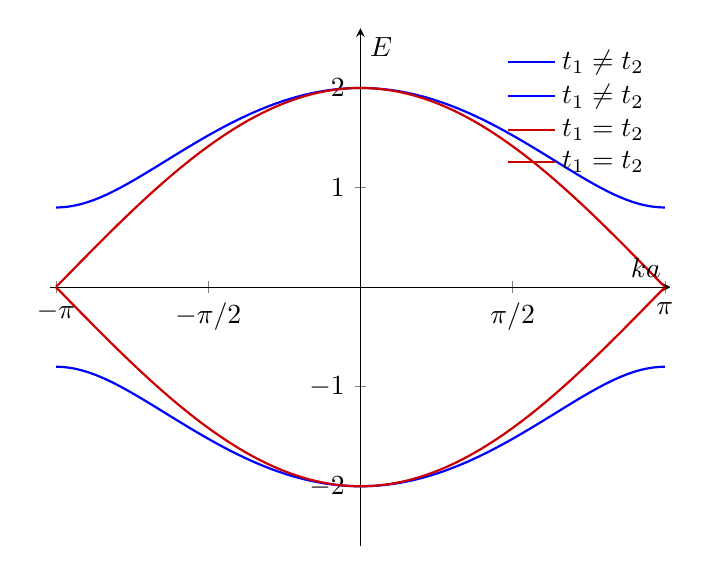
\begin{tikzpicture}
\begin{axis}[
  width=0.78\textwidth,
  xlabel={$ka$},
  ylabel={$E$},
  xmin=-3.2,xmax=3.2,
  ymin=-2.6,ymax=2.6,
  axis lines=middle,
  xtick={-3.1416,-1.5708,0,1.5708,3.1416},
  xticklabels={$-\pi$,$-\pi/2$,$0$,$\pi/2$,$\pi$},
  samples=300,
  domain=-3.1416:3.1416,
  legend style={draw=none,fill=none,at={(0.98,0.98)},anchor=north east}
]
\addplot[thick,blue] {sqrt(0.6^2+1.4^2+2*0.6*1.4*cos(deg(x)))};
\addplot[thick,blue] {-sqrt(0.6^2+1.4^2+2*0.6*1.4*cos(deg(x)))};
\addplot[thick,red!80!black] {sqrt(1+1+2*cos(deg(x)))};
\addplot[thick,red!80!black] {-sqrt(1+1+2*cos(deg(x)))};
\legend{\(t_1\neq t_2\),\(t_1\neq t_2\),\(t_1=t_2\),\(t_1=t_2\)}
\end{axis}
\end{tikzpicture}
\caption{Dispersión del modelo SSH. En azul, el caso gapped \(t_1\neq t_2\). En rojo, el caso crítico \(t_1=t_2\), donde el gap se cierra en \(ka=\pi\).}
\label{c01:fig:ssh-disp}
\end{figure}

\section{Linealización alrededor del punto crítico}

\subsection{Expansión alrededor de k0 = pi/a}

Escribimos
\begin{equation}
k = \frac{\pi}{a}+q,
\qquad |q a|\ll 1.
\end{equation}

Entonces
\begin{align}
\cos(ka)
&=
\cos(\pi+qa)
=
-\cos(qa)
\approx -1,
\\
\sin(ka)
&=
\sin(\pi+qa)
=
-\sin(qa)
\approx -qa.
\end{align}

Sustituyendo en \eqref{c01:eq:ssh-dxdy},
\begin{align}
d_x(k)
&\approx t_1-t_2,
\\
d_y(k)
&\approx -t_2\, a\, q.
\end{align}

Por tanto, cerca del punto crítico:
\begin{equation}
H(q)\approx (t_1-t_2)\sigma_x - t_2 a q\,\sigma_y.
\label{c01:eq:ssh-linear}
\end{equation}

\subsection{Caso exactamente crítico}

Si \(t_1=t_2=t\), el primer término desaparece y queda
\begin{equation}
H_{\text{crit}}(q)\approx - t a q\, \sigma_y.
\label{c01:eq:ssh-critical-linear}
\end{equation}

Eso es ya un Hamiltoniano lineal en el momento, exactamente lo que esperamos de una teoría de Dirac sin masa en \(1+1\).

\subsection{Interpretación del término t1 - t2}

Definimos
\begin{equation}
m \equiv t_1-t_2,
\qquad
v \equiv t a.
\end{equation}

Entonces \eqref{c01:eq:ssh-linear} se escribe como
\begin{equation}
H(q)\approx m\,\sigma_x - v q\,\sigma_y.
\label{c01:eq:ssh-massive-dirac}
\end{equation}

Esta es la forma estándar de un Hamiltoniano de Dirac masivo en \(1D\): un término lineal en el momento más un término de masa controlable.

\section{Relación con la ecuación de Dirac}

\subsection{Estructura relativista efectiva}

Si promovemos \(q\to -\ii \partial_x\), la ecuación efectiva toma la forma
\begin{equation}
\ii \partial_t \Psi =
\left(
m\,\sigma_x + \ii v\,\sigma_y \partial_x
\right)\Psi.
\label{c01:eq:ssh-dirac-real}
\end{equation}

Con una redefinición conveniente de matrices, esto es equivalente a una ecuación de Dirac en \(1+1\):
\begin{equation}
\left(
\ii \gamma^\mu \partial_\mu - m
\right)\Psi=0.
\end{equation}

Lo importante aquí no es la representación específica de las matrices gamma, sino el hecho estructural:

\begin{enumerate}[leftmargin=*]
  \item el grado de libertad de subred produce un espinor de dos componentes;
  \item la linealización del Hamiltoniano produce un operador de primer orden;
  \item la diferencia \(t_1-t_2\) actúa exactamente como una masa efectiva.
\end{enumerate}

\subsection{Espectro efectivo}

Del Hamiltoniano \eqref{c01:eq:ssh-massive-dirac}, el espectro es
\begin{equation}
E_\pm(q)=\pm \sqrt{m^2+v^2 q^2}.
\label{c01:eq:ssh-effective-disp}
\end{equation}

Si \(m=0\), obtenemos una dispersión lineal gapless. Si \(m\neq 0\), se abre un gap de tamaño
\begin{equation}
\Delta = 2|m| = 2|t_1-t_2|.
\end{equation}

\begin{figure}[ht]
\centering
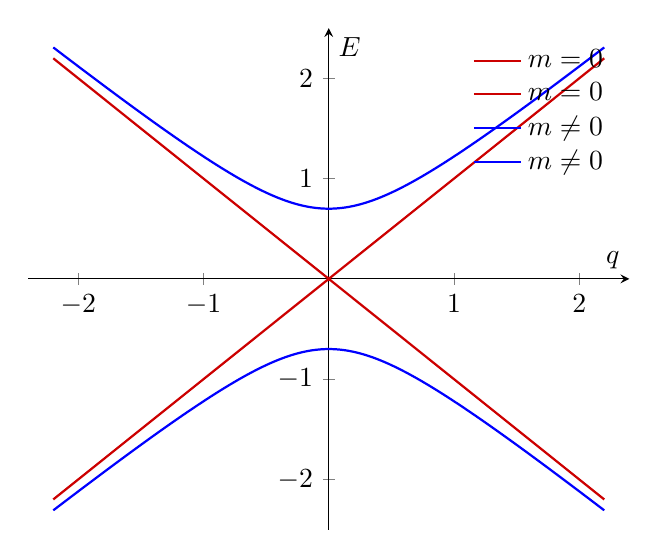
\begin{tikzpicture}
\begin{axis}[
  width=0.76\textwidth,
  xlabel={$q$},
  ylabel={$E$},
  xmin=-2.4,xmax=2.4,
  ymin=-2.5,ymax=2.5,
  axis lines=middle,
  samples=250,
  domain=-2.2:2.2,
  legend style={draw=none,fill=none,at={(0.98,0.98)},anchor=north east}
]
\addplot[thick,red!80!black] {abs(x)};
\addplot[thick,red!80!black] {-abs(x)};
\addplot[thick,blue] {sqrt(0.7^2+x^2)};
\addplot[thick,blue] {-sqrt(0.7^2+x^2)};
\legend{\(m=0\),\(m=0\),\(m\neq 0\),\(m\neq 0\)}
\end{axis}
\end{tikzpicture}
\caption{Dispersión efectiva del modelo linealizado. El caso crítico \(m=0\) produce un cono lineal en \(1D\); el caso \(m\neq 0\) abre una brecha.}
\label{c01:fig:ssh-effective}
\end{figure}

\section{Interpretación topológica mínima}

Aunque aquí estamos usando el modelo sobre todo como ejemplo de Dirac emergente, el SSH también enseña una lección topológica importante. Los dos regímenes:
\begin{equation}
t_1>t_2
\qquad \text{y} \qquad
t_2>t_1
\end{equation}
no son simplemente dos versiones cuantitativas del mismo sistema; corresponden a fases topológicas distintas.

El punto crítico \(t_1=t_2\) separa esas dos fases. En el lenguaje efectivo, eso se refleja en el cambio de signo de la masa:
\begin{equation}
m=t_1-t_2.
\end{equation}

Esto es pedagógicamente muy valioso para el proyecto, porque más adelante en grafeno, y todavía más en Dirac/Weyl 3D, veremos que cambiar el signo de un término de masa o romper una simetría puede cambiar por completo la naturaleza de la fase.

\section{Qué enseña SSH para el proyecto}

El modelo SSH deja ya fijadas varias lecciones centrales:

\begin{enumerate}[leftmargin=*]
  \item una red discreta con estructura interna puede producir espinores efectivos;
  \item una teoría tipo Dirac emerge por linealización alrededor de un punto de cierre del gap;
  \item la masa efectiva se controla con un parámetro microscópico sencillo;
  \item una transición de fase puede leerse como cambio de signo del término de masa.
\end{enumerate}

En otras palabras: SSH es el laboratorio mínimo donde aparecen, en forma limpia, pseudospín, cierre del gap, masa efectiva y Dirac emergente.

\section{Mapa de la derivación}

\begin{figure}[ht]
\centering
\begin{tikzpicture}[
  node distance=8mm and 9mm,
  every node/.style={font=\small},
  box/.style={draw,rounded corners,thick,align=center,minimum width=3.2cm,minimum height=1cm,fill=blue!6},
  arr/.style={-{Latex[length=3mm]},thick}
]
  \node[box] (a) {Cadena con dos sitios\\ por celda \(A/B\)};
  \node[box, right=of a] (b) {Hamiltoniano SSH\\ \(t_1,t_2\)};
  \node[box, right=of b] (c) {Hamiltoniano de Bloch\\ \(H(k)\)};
  \node[box, below=of b] (d) {Cierre del gap\\ \(t_1=t_2,\; k=\pi/a\)};
  \node[box, left=of d] (e) {Linealización\\ \(k=\pi/a+q\)};
  \node[box, right=of d] (f) {Dirac 1D\\ \(H\approx m\sigma_x-vq\sigma_y\)};

  \draw[arr] (a) -- (b);
  \draw[arr] (b) -- (c);
  \draw[arr] (c) -- (d);
  \draw[arr] (d) -- (e);
  \draw[arr] (d) -- (f);
\end{tikzpicture}
\caption{Ruta conceptual del capítulo SSH.}
\label{c01:fig:ssh-roadmap}
\end{figure}

\section{Dónde encaja dentro del programa}

Este documento cumple exactamente el primer paso sugerido en tu programa:

\begin{enumerate}[leftmargin=*]
  \item reemplaza la cadena unidimensional simple por el ejemplo correcto, el SSH;
  \item muestra cómo aparece una estructura espinorial efectiva en \(1D\);
  \item introduce la masa efectiva de forma controlable;
  \item prepara el lenguaje que luego se reutiliza en grafeno y en modelos \(3D\).
\end{enumerate}

La secuencia del proyecto queda ahora mucho más ordenada:

\begin{enumerate}[leftmargin=*]
  \item SSH \(\rightarrow\) Dirac \(1+1\),
  \item grafeno \(\rightarrow\) Dirac \(2+1\),
  \item semimetales \(\rightarrow\) Dirac/Weyl en \(3D\),
  \item luego Nielsen--Ninomiya y, si conviene, tiempo discreto.
\end{enumerate}

% % Importado desde: 2026-03-28_Derivacion_Grafeno_a_Dirac.tex
\chapter{Derivacion Pedagogica: --- De la red honeycomb de grafeno al Hamiltoniano de Dirac en \(2+1\)}
\label{ch:derivacion-grafeno-a-dirac}

\section{Objetivo}

La meta de este documento es derivar, de manera lenta y explicita, como la ecuacion efectiva de Dirac aparece en grafeno a partir de un modelo tight-binding de primeros vecinos sobre la red honeycomb. La idea es dejar un texto autocontenido, con figuras y cuentas intermedias, que sirva como base de estudio antes de pasar a una formulacion mas tecnica de materiales de Dirac y Weyl en tres dimensiones.

La cadena conceptual que vamos a recorrer es:
\[
\begin{aligned}
\text{red honeycomb}
&\longrightarrow
\text{Hamiltoniano tight-binding}
\longrightarrow
\text{matriz de Bloch } H(\vk)
\\
&\longrightarrow
\text{puntos } K,K'
\longrightarrow
\text{expansion lineal}
\longrightarrow
\text{Hamiltoniano de Dirac efectivo.}
\end{aligned}
\]

\section{Panorama general}

Grafeno tiene dos ingredientes estructurales esenciales:

\begin{enumerate}[leftmargin=*]
  \item la red no es una red de Bravais simple, sino una red de Bravais triangular con una base de dos atomos;
  \item esos dos atomos por celda unitaria definen dos subredes, tradicionalmente llamadas \(A\) y \(B\).
\end{enumerate}

Como el electron puede saltar entre primeros vecinos de \(A\) a \(B\), el Hamiltoniano natural tiene una estructura \(2\times 2\) en el espacio de subred. Esa estructura matricial es la semilla del pseudospin de grafeno y es la razon por la que las matrices de Pauli aparecen naturalmente en la teoria efectiva.

\section{La red honeycomb en espacio real}

\subsection{Subredes y vectores de primeros vecinos}

Tomamos una convencion sencilla para los tres vectores que conectan un sitio de la subred \(A\) con sus tres vecinos mas cercanos de la subred \(B\):
\begin{equation}
\vdelta_1 = a(0,-1),
\qquad
\vdelta_2 = a\left(\frac{\sqrt{3}}{2},\frac{1}{2}\right),
\qquad
\vdelta_3 = a\left(-\frac{\sqrt{3}}{2},\frac{1}{2}\right),
\label{eq:deltas}
\end{equation}
donde \(a\) es la distancia entre atomos vecinos.

Con esta eleccion, dos vectores primitivos de la red de Bravais triangular asociada a la subred \(A\) pueden tomarse como
\begin{equation}
\va_1 = \vdelta_2 - \vdelta_3 = a(\sqrt{3},0),
\qquad
\va_2 = \vdelta_3 - \vdelta_1 = a\left(-\frac{\sqrt{3}}{2},\frac{3}{2}\right).
\label{eq:primitive-real}
\end{equation}

\begin{figure}[ht]
\centering
\begin{tikzpicture}[scale=1.45,>=Latex]
  \coordinate (A0) at (0,0);
  \coordinate (B1) at (0,-1);
  \coordinate (B2) at (0.866,0.5);
  \coordinate (B3) at (-0.866,0.5);
  \coordinate (Ar) at (1.732,0);
  \coordinate (Al) at (-1.732,0);
  \coordinate (Aul) at (-0.866,1.5);
  \coordinate (Aur) at (0.866,1.5);
  \coordinate (Adl) at (-0.866,-1.5);
  \coordinate (Adr) at (0.866,-1.5);
  \coordinate (Br1) at (1.732,1);
  \coordinate (Br2) at (1.732,-1);
  \coordinate (Bl1) at (-1.732,1);
  \coordinate (Bl2) at (-1.732,-1);

  \foreach \p/\q in {
    A0/B1,A0/B2,A0/B3,
    Ar/B2,Ar/Br1,Ar/Br2,
    Al/B3,Al/Bl1,Al/Bl2,
    Aul/B2,Aul/B3,Aul/Bl1,
    Aur/B2,Aur/B3,Aur/Br1,
    Adl/B1,Adl/B3,Adl/Bl2,
    Adr/B1,Adr/B2,Adr/Br2}
    \draw[gray!70,line width=0.8pt] (\p) -- (\q);

  \foreach \p in {A0,Ar,Al,Aul,Aur,Adl,Adr}
    \fill[blue!70] (\p) circle (2.2pt);
  \foreach \p in {B1,B2,B3,Br1,Br2,Bl1,Bl2}
    \fill[orange!85!black] (\p) circle (2.2pt);

  \node[above left=1pt of A0] {$A$};
  \node[right=1pt of B2] {$B$};

  \draw[->,very thick,red!75!black] (A0) -- (B1) node[midway,right] {$\vdelta_1$};
  \draw[->,very thick,red!75!black] (A0) -- (B2) node[midway,above right] {$\vdelta_2$};
  \draw[->,very thick,red!75!black] (A0) -- (B3) node[midway,above left] {$\vdelta_3$};

  \draw[->,thick,blue!80!black] (A0) -- (Ar) node[midway,below] {$\va_1$};
  \draw[->,thick,blue!80!black] (A0) -- (Aul) node[midway,left] {$\va_2$};

  \node[below left] at (-2.15,-1.85) {\footnotesize subred $A$};
  \fill[blue!70] (-2.48,-1.83) circle (2pt);
  \node[below left] at (-2.15,-2.12) {\footnotesize subred $B$};
  \fill[orange!85!black] (-2.48,-2.10) circle (2pt);
\end{tikzpicture}
\caption{Patch local de la red honeycomb de grafeno. Los sitios azules forman la subred \(A\) y los naranjas la subred \(B\). Los vectores \(\vdelta_i\) conectan primeros vecinos \(A\to B\), mientras que \(\va_1,\va_2\) generan la red de Bravais subyacente.}
\label{fig:honeycomb}
\end{figure}

\subsection{Por que aparecen dos componentes en la funcion de onda}

Como hay dos sitios distintos por celda, la amplitud de la funcion de onda debe llevar dos componentes:
\begin{equation}
\Psi(\vR) =
\begin{pmatrix}
\psi_A(\vR)\\[4pt]
\psi_B(\vR)
\end{pmatrix}.
\end{equation}

Esta estructura de dos componentes no es el espin real del electron. Es un grado de libertad de subred, y por eso se le llama \textit{pseudospin}. Mas adelante las matrices de Pauli \(\sigma_x,\sigma_y,\sigma_z\) actuaran sobre este espacio \(A/B\).

\section{Hamiltoniano tight-binding}

\subsection{El modelo minimo}

En el modelo mas simple retenemos solo saltos entre primeros vecinos y un unico parametro de hopping \(t\). El Hamiltoniano es
\begin{equation}
H = -t \sum_{\vR}\sum_{j=1}^3
\left(
a_{\vR}^\dagger b_{\vR+\vdelta_j}
+ b_{\vR+\vdelta_j}^\dagger a_{\vR}
\right),
\label{eq:tb-real}
\end{equation}
donde:

\begin{enumerate}[leftmargin=*]
  \item \(a_{\vR}^\dagger\) crea un electron en la subred \(A\) de la celda \(\vR\);
  \item \(b_{\vR+\vdelta_j}^\dagger\) crea un electron en uno de los tres vecinos \(B\);
  \item el signo menos es la convencion usual del tight-binding para que la banda de conduccion y valencia queden simetricas alrededor de cero.
\end{enumerate}

\subsection{Lectura fisica de la ecuacion}

La expresion \eqref{eq:tb-real} dice algo muy concreto: un electron sentado en \(A\) puede saltar a cualquiera de sus tres vecinos \(B\), y viceversa. Toda la estructura no trivial de grafeno aparece porque esos tres caminos interfieren entre si cuando pasamos al espacio de momentos.

\section{Paso al espacio recíproco}

\subsection{Transformadas de Fourier}

Definimos
\begin{equation}
a_{\vR} = \frac{1}{\sqrt{N}}\sum_{\vk}\ee^{\ii \vk\cdot\vR} a_{\vk},
\qquad
b_{\vR+\vdelta_j} = \frac{1}{\sqrt{N}}\sum_{\vk}\ee^{\ii \vk\cdot(\vR+\vdelta_j)} b_{\vk},
\label{eq:fourier}
\end{equation}
con \(N\) el numero de celdas unitarias.

Sustituyendo \eqref{eq:fourier} en \eqref{eq:tb-real} se obtiene
\begin{align}
H
&=
-t \sum_{\vR}\sum_{j=1}^3
\left[
\left(\frac{1}{\sqrt{N}}\sum_{\vk}\ee^{-\ii \vk\cdot\vR}a_{\vk}^\dagger\right)
\left(\frac{1}{\sqrt{N}}\sum_{\vk'}\ee^{\ii \vk'\cdot(\vR+\vdelta_j)}b_{\vk'}\right)
+ \text{h.c.}
\right]
\nonumber\\[4pt]
&=
-\frac{t}{N}\sum_{\vR}\sum_{j=1}^3\sum_{\vk,\vk'}
\ee^{\ii(\vk'-\vk)\cdot\vR}\,
\ee^{\ii \vk'\cdot\vdelta_j}\,
a_{\vk}^\dagger b_{\vk'}
+ \text{h.c.}
\label{eq:before-orthogonality}
\end{align}

Ahora usamos la identidad de ortogonalidad
\begin{equation}
\sum_{\vR}\ee^{\ii(\vk'-\vk)\cdot\vR}=N\,\delta_{\vk,\vk'}.
\end{equation}

Con esto, la suma en \(\vR\) fuerza \(\vk'=\vk\), y queda
\begin{equation}
H=
-t\sum_{\vk}\sum_{j=1}^3
\left(
\ee^{\ii \vk\cdot\vdelta_j} a_{\vk}^\dagger b_{\vk}
+ \ee^{-\ii \vk\cdot\vdelta_j} b_{\vk}^\dagger a_{\vk}
\right).
\label{eq:hk-sum}
\end{equation}

\subsection{La matriz de Bloch}

Introducimos la funcion estructural
\begin{equation}
f(\vk)=\sum_{j=1}^3 \ee^{\ii \vk\cdot\vdelta_j}.
\label{eq:fk}
\end{equation}

Entonces \eqref{eq:hk-sum} se escribe como
\begin{equation}
H = \sum_{\vk}
\begin{pmatrix}
a_{\vk}^\dagger & b_{\vk}^\dagger
\end{pmatrix}
\begin{pmatrix}
0 & -t f(\vk)\\
-t f^*(\vk) & 0
\end{pmatrix}
\begin{pmatrix}
a_{\vk}\\
b_{\vk}
\end{pmatrix}.
\label{eq:bloch-matrix}
\end{equation}

Asi, el Hamiltoniano de una sola particula es
\begin{equation}
H(\vk)=
\begin{pmatrix}
0 & -t f(\vk)\\
-t f^*(\vk) & 0
\end{pmatrix}.
\label{eq:Hk}
\end{equation}

\section{Bandas de energia}

\subsection{Calculo de autovalores}

Los autovalores se obtienen de
\begin{equation}
\det\!\big(H(\vk)-E I\big)=0.
\end{equation}

Como
\begin{equation}
\det
\begin{pmatrix}
-E & -t f(\vk)\\
-t f^*(\vk) & -E
\end{pmatrix}
= E^2 - t^2 |f(\vk)|^2,
\end{equation}
resulta
\begin{equation}
E_\pm(\vk)=\pm t |f(\vk)|.
\label{eq:dispersion-general}
\end{equation}

Esto ya muestra dos cosas fundamentales:

\begin{enumerate}[leftmargin=*]
  \item hay dos bandas, una de conduccion y una de valencia;
  \item el contacto entre ellas ocurre cuando \(f(\vk)=0\).
\end{enumerate}

\subsection{Forma explicita de f(k)}

Usando los vectores \eqref{eq:deltas},
\begin{align}
f(\vk)
&=
\ee^{-\ii a k_y}
+ \ee^{\ii\left(\frac{\sqrt{3}}{2}a k_x+\frac{1}{2}a k_y\right)}
+ \ee^{\ii\left(-\frac{\sqrt{3}}{2}a k_x+\frac{1}{2}a k_y\right)}
\nonumber\\[4pt]
&=
\ee^{-\ii a k_y}
+ 2\,\ee^{\ii a k_y/2}\cos\!\left(\frac{\sqrt{3}}{2}a k_x\right).
\label{eq:fk-explicit}
\end{align}

Al tomar el modulo al cuadrado se obtiene
\begin{equation}
|f(\vk)|^2
=
1
+4\cos^2\!\left(\frac{\sqrt{3}}{2}a k_x\right)
+4\cos\!\left(\frac{\sqrt{3}}{2}a k_x\right)\cos\!\left(\frac{3}{2}a k_y\right).
\label{eq:fk-mod}
\end{equation}

Por tanto,
\begin{equation}
E_\pm(\vk)=
\pm t
\sqrt{
1
+4\cos^2\!\left(\frac{\sqrt{3}}{2}a k_x\right)
+4\cos\!\left(\frac{\sqrt{3}}{2}a k_x\right)\cos\!\left(\frac{3}{2}a k_y\right)
}.
\label{eq:graphene-dispersion}
\end{equation}

\section{La zona de Brillouin y los puntos de Dirac}

\subsection{Donde se tocan las bandas}

Las bandas se tocan cuando \(f(\vk)=0\). Una solucion especialmente importante es
\begin{equation}
\vK=\left(\frac{4\pi}{3\sqrt{3}a},0\right),
\qquad
\vK'=\left(-\frac{4\pi}{3\sqrt{3}a},0\right).
\label{eq:KKp}
\end{equation}

Verificacion rapida en \(\vK\):
\begin{equation}
f(\vK)
=
1+\ee^{\ii 2\pi/3}+\ee^{-\ii 2\pi/3}
=1+2\cos(2\pi/3)=0.
\end{equation}

La misma cancelacion ocurre en \(\vK'\). Estos son dos puntos no equivalentes de la primera zona de Brillouin y son justamente los puntos de Dirac.

\begin{figure}[ht]
\centering
\begin{tikzpicture}[scale=1.2,>=Latex]
  \def\R{2.3}
  \foreach \ang in {0,60,...,300}
    \coordinate (P\ang) at (\ang:\R);

  \draw[thick] (P0)--(P60)--(P120)--(P180)--(P240)--(P300)--cycle;
  \draw[->] (-2.8,0) -- (2.8,0) node[right] {$k_x$};
  \draw[->] (0,-2.5) -- (0,2.7) node[above] {$k_y$};

  \fill (0,0) circle (2pt);
  \node[below left] at (0,0) {$\Gamma$};

  \coordinate (K) at (1.53,0);
  \coordinate (Kp) at (-1.53,0);
  \fill[red!80!black] (K) circle (2.2pt);
  \fill[red!80!black] (Kp) circle (2.2pt);
  \node[below] at (K) {$K$};
  \node[below] at (Kp) {$K'$};

  \draw[blue!80!black,thick,->] (K) -- ++(0.55,0.45) node[above right] {$\vq$};
  \draw[blue!80!black,thick,->] (Kp) -- ++(-0.55,0.45) node[above left] {$\vq$};

  \draw[gray!60,dashed] (K) circle (0.38);
  \draw[gray!60,dashed] (Kp) circle (0.38);

  \node[align=center] at (0,2.15) {\footnotesize Primera zona de Brillouin\\ \footnotesize y regiones de expansion de baja energia};
\end{tikzpicture}
\caption{Primera zona de Brillouin esquematica para grafeno. Los puntos \(K\) y \(K'\) son los puntos no equivalentes donde se anulan simultaneamente las bandas y alrededor de los cuales se hace la expansion lineal \(\vk=\vK+\vq\) o \(\vk=\vK'+\vq\).}
\label{fig:bz}
\end{figure}

\subsection{Significado fisico}

La anulacion de \(f(\vk)\) no es accidental. Es una interferencia destructiva exacta entre los tres caminos de hopping desde un sitio de la subred \(A\) hacia los tres vecinos \(B\). Esa cancelacion obliga a que las bandas se toquen sin abrir gap en los puntos \(K\) y \(K'\).

\section{Expansion alrededor de K}

\subsection{Paso algebraico principal}

Escribimos
\begin{equation}
\vk=\vK+\vq,
\qquad |\vq| \ll |\vK|.
\end{equation}

Entonces
\begin{align}
f(\vK+\vq)
&=
\sum_{j=1}^3 \ee^{\ii (\vK+\vq)\cdot\vdelta_j}
=
\sum_{j=1}^3 \ee^{\ii \vK\cdot\vdelta_j}\ee^{\ii \vq\cdot\vdelta_j}.
\end{align}

Como \(|\vq\cdot\vdelta_j|\ll 1\), hacemos expansion a primer orden:
\begin{equation}
\ee^{\ii \vq\cdot\vdelta_j}\approx 1+\ii \vq\cdot\vdelta_j.
\end{equation}

Luego
\begin{equation}
f(\vK+\vq)\approx
\sum_{j=1}^3 \ee^{\ii \vK\cdot\vdelta_j}
+ \ii \sum_{j=1}^3 \ee^{\ii \vK\cdot\vdelta_j} \vq\cdot\vdelta_j.
\label{eq:f-expand-general}
\end{equation}

El primer termino se anula porque \(f(\vK)=0\). Por tanto
\begin{equation}
f(\vK+\vq)\approx
\ii \sum_{j=1}^3 \ee^{\ii \vK\cdot\vdelta_j} \vq\cdot\vdelta_j.
\label{eq:linear-term-only}
\end{equation}

\subsection{Cuenta explicita}

Para nuestra convencion,
\begin{equation}
\ee^{\ii \vK\cdot\vdelta_1}=1,
\qquad
\ee^{\ii \vK\cdot\vdelta_2}=\ee^{\ii 2\pi/3},
\qquad
\ee^{\ii \vK\cdot\vdelta_3}=\ee^{-\ii 2\pi/3}.
\end{equation}

Ademas,
\begin{align}
\vq\cdot\vdelta_1 &= -a q_y,
\nonumber\\
\vq\cdot\vdelta_2 &= a\left(\frac{\sqrt{3}}{2}q_x+\frac{1}{2}q_y\right),
\nonumber\\
\vq\cdot\vdelta_3 &= a\left(-\frac{\sqrt{3}}{2}q_x+\frac{1}{2}q_y\right).
\end{align}

Sustituyendo en \eqref{eq:linear-term-only},
\begin{align}
f(\vK+\vq)
&\approx
\ii \Bigg[
(-a q_y)
+ \ee^{\ii 2\pi/3}a\left(\frac{\sqrt{3}}{2}q_x+\frac{1}{2}q_y\right)
+ \ee^{-\ii 2\pi/3}a\left(-\frac{\sqrt{3}}{2}q_x+\frac{1}{2}q_y\right)
\Bigg].
\end{align}

Agrupamos \(q_x\) y \(q_y\) por separado:
\begin{align}
f(\vK+\vq)
&\approx
\ii a
\left[
\frac{\sqrt{3}}{2}\left(\ee^{\ii 2\pi/3}-\ee^{-\ii 2\pi/3}\right)q_x
+
\left(
-1+\frac{1}{2}\ee^{\ii 2\pi/3}+\frac{1}{2}\ee^{-\ii 2\pi/3}
\right)q_y
\right].
\end{align}

Usamos
\begin{equation}
\ee^{\ii 2\pi/3}-\ee^{-\ii 2\pi/3}=2\ii \sin(2\pi/3)=\ii\sqrt{3},
\end{equation}
y
\begin{equation}
\ee^{\ii 2\pi/3}+\ee^{-\ii 2\pi/3}=2\cos(2\pi/3)=-1.
\end{equation}

Entonces
\begin{align}
f(\vK+\vq)
&\approx
\ii a
\left[
\frac{\sqrt{3}}{2}(\ii\sqrt{3})q_x
+\left(-1-\frac{1}{2}\right)q_y
\right]
\nonumber\\[4pt]
&=
\ii a
\left[
\frac{3\ii}{2}q_x - \frac{3}{2}q_y
\right]
\nonumber\\[4pt]
&=
-\frac{3a}{2}(q_x+\ii q_y).
\label{eq:fK-final}
\end{align}

\subsection{Hamiltoniano efectivo cerca de K}

Insertando \eqref{eq:fK-final} en \eqref{eq:Hk},
\begin{equation}
H_K(\vq)
\approx
\frac{3at}{2}
\begin{pmatrix}
0 & q_x+\ii q_y\\
q_x-\ii q_y & 0
\end{pmatrix}.
\end{equation}

Definimos la velocidad de Fermi
\begin{equation}
v_F=\frac{3at}{2\hbar}.
\label{eq:vf}
\end{equation}

Entonces
\begin{equation}
H_K(\vq)
=
\hbar v_F
\begin{pmatrix}
0 & q_x+\ii q_y\\
q_x-\ii q_y & 0
\end{pmatrix}.
\label{eq:HK-matrix}
\end{equation}

En terminos de matrices de Pauli,
\begin{equation}
H_K(\vq)=\hbar v_F\,(q_x \sigma_x - q_y \sigma_y).
\label{eq:HK-pauli}
\end{equation}

Con una simple redefinicion unitaria de la base de subred, esta forma es equivalente a la version mas difundida
\begin{equation}
H_K(\vq)\sim \hbar v_F\,(q_x \sigma_x + q_y \sigma_y).
\label{eq:HK-standard}
\end{equation}

El punto importante no es el signo de una convencion de base, sino que el Hamiltoniano es lineal en \(\vq\) y tiene estructura exacta de Dirac sin masa en \(2+1\).

\section{Expansion alrededor de K'}

Ahora escribimos
\begin{equation}
\vk=\vK'+\vq,
\qquad
\vK'=-\vK.
\end{equation}

Repitiendo la expansion se obtiene
\begin{equation}
f(\vK'+\vq)\approx \frac{3a}{2}(q_x-\ii q_y).
\label{eq:fKp-final}
\end{equation}

Por tanto,
\begin{equation}
H_{K'}(\vq)
\approx
-\hbar v_F
\begin{pmatrix}
0 & q_x-\ii q_y\\
q_x+\ii q_y & 0
\end{pmatrix}.
\label{eq:HKp-matrix}
\end{equation}

De nuevo, dependiendo de la convencion de base, esto suele escribirse en forma compacta como
\begin{equation}
H_\tau(\vq)=\hbar v_F(\tau q_x \sigma_x + q_y \sigma_y),
\qquad \tau=\pm 1,
\label{eq:valley-compact}
\end{equation}
donde \(\tau=+1\) corresponde a \(K\) y \(\tau=-1\) a \(K'\).

\section{La dispersion lineal y el cono de Dirac}

\subsection{Autovalores de la teoria efectiva}

Para cualquiera de las dos valles, el Hamiltoniano efectivo tiene autovalores
\begin{equation}
E_\pm(\vq)=\pm \hbar v_F |\vq|.
\label{eq:dirac-dispersion}
\end{equation}

Esto es una dispersion lineal, no cuadratica. Cerca del punto de contacto, las bandas forman un cono superior y otro inferior: el famoso cono de Dirac.

\begin{figure}[ht]
\centering
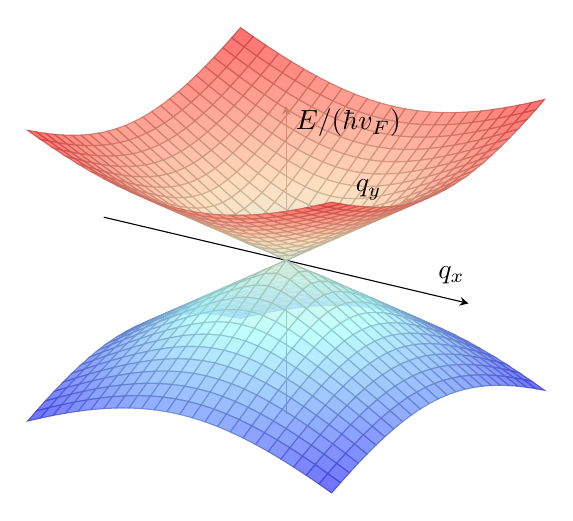
\begin{tikzpicture}
\begin{axis}[
  width=0.78\textwidth,
  view={35}{26},
  axis lines=center,
  xlabel={$q_x$},
  ylabel={$q_y$},
  zlabel={$E/(\hbar v_F)$},
  xmin=-1.2,xmax=1.2,
  ymin=-1.2,ymax=1.2,
  zmin=-1.5,zmax=1.5,
  ticks=none,
  colormap={mycmap}{
    color=(blue!70)
    color=(cyan!30)
    color=(orange!30)
    color=(red!70)
  },
  samples=25,
  domain=-1:1,
  y domain=-1:1
]
\addplot3[surf,opacity=0.82] {sqrt(x^2+y^2)};
\addplot3[surf,opacity=0.82] {-sqrt(x^2+y^2)};
\end{axis}
\end{tikzpicture}
\caption{Dispersion efectiva cerca de un punto de Dirac. La energia es lineal en \(|\vq|\), de modo que las bandas de conduccion y valencia forman un doble cono que se toca en \(E=0\).}
\label{fig:cone}
\end{figure}

\subsection{Interpretacion}

La ecuacion \eqref{eq:dirac-dispersion} es la firma de fermiones relativistas efectivos sin masa. La velocidad de la luz \(c\) de la teoria relativista es reemplazada aqui por la velocidad de Fermi \(v_F\), y las matrices de Pauli actuan sobre el pseudospin de subred en lugar del espin real.

\section{Como se lee esto como ecuacion de Dirac}

\subsection{Del Hamiltoniano a la ecuacion de movimiento}

La ecuacion de Schrodinger efectiva es
\begin{equation}
\ii \hbar \,\partial_t \Psi = H_\tau \Psi.
\end{equation}

Usando \eqref{eq:valley-compact},
\begin{equation}
\ii \hbar \,\partial_t \Psi
=
\hbar v_F(\tau q_x \sigma_x + q_y \sigma_y)\Psi.
\end{equation}

Al pasar a espacio real, \(q_x\to -\ii\partial_x\) y \(q_y\to -\ii\partial_y\), de modo que
\begin{equation}
\ii \partial_t \Psi
=
-\ii v_F(\tau \sigma_x \partial_x + \sigma_y \partial_y)\Psi.
\label{eq:dirac-real-space}
\end{equation}

Esta es exactamente una ecuacion de Dirac sin masa en \(2+1\), escrita en una representacion adaptada al problema de grafeno.

\subsection{Que representa cada simbolo}

\begin{center}
\begin{tabular}{p{0.28\textwidth}p{0.58\textwidth}}
\toprule
\textbf{Objeto} & \textbf{Interpretacion en grafeno} \\
\midrule
\(\Psi\) & espinor de dos componentes en subred \(A/B\) \\
\(\sigma_x,\sigma_y,\sigma_z\) & matrices de Pauli sobre el pseudospin \\
\(\tau=\pm 1\) & indice de valle, asociado a \(K\) y \(K'\) \\
\(v_F\) & velocidad de Fermi efectiva \\
\(E=\pm \hbar v_F |\vq|\) & dispersion lineal tipo fermion sin masa \\
\bottomrule
\end{tabular}
\end{center}

\section{Resumen paso por paso}

\begin{enumerate}[leftmargin=*]
  \item La red honeycomb se descompone en dos subredes, \(A\) y \(B\).
  \item Eso obliga a usar una funcion de onda de dos componentes.
  \item El modelo tight-binding de primeros vecinos produce una matriz \(2\times 2\) en el espacio de subred.
  \item En espacio recíproco, toda la informacion geometrica queda contenida en \(f(\vk)=\sum_j \ee^{\ii \vk\cdot\vdelta_j}\).
  \item Las bandas se tocan cuando \(f(\vk)=0\), lo que ocurre en \(K\) y \(K'\).
  \item Al expandir \(\vk=\vK+\vq\) o \(\vk=\vK'+\vq\), el Hamiltoniano se vuelve lineal en \(\vq\).
  \item Esa expansion lineal es el Hamiltoniano de Dirac efectivo de grafeno.
\end{enumerate}

\begin{figure}[ht]
\centering
\begin{tikzpicture}[
  node distance=8mm and 10mm,
  every node/.style={font=\small},
  box/.style={draw,rounded corners,thick,align=center,minimum width=3.1cm,minimum height=0.95cm,fill=blue!6},
  arr/.style={-{Latex[length=3mm]},thick}
]
  \node[box] (r1) {Red honeycomb\\ dos subredes \(A/B\)};
  \node[box, right=of r1] (r2) {Hamiltoniano\\ tight-binding};
  \node[box, right=of r2] (r3) {Matriz de Bloch\\ \(H(\vk)\)};
  \node[box, below=of r2] (r4) {Ceros de \(f(\vk)\)\\ puntos \(K\) y \(K'\)};
  \node[box, left=of r4] (r5) {Expansion\\ \(\vk=\vK+\vq\)};
  \node[box, right=of r4] (r6) {Hamiltoniano lineal\\ \(\hbar v_F\,\bm{\sigma}\cdot\vq\)};

  \draw[arr] (r1) -- (r2);
  \draw[arr] (r2) -- (r3);
  \draw[arr] (r3) -- (r4);
  \draw[arr] (r4) -- (r5);
  \draw[arr] (r4) -- (r6);
\end{tikzpicture}
\caption{Mapa conceptual de la derivacion.}
\label{fig:flow}
\end{figure}

\section{Que dejamos listo para el siguiente paso}

Con esta derivacion ya quedan establecidas las piezas que hacen falta para avanzar luego hacia materiales de Dirac y Weyl:

\begin{enumerate}[leftmargin=*]
  \item el origen del pseudospin;
  \item la emergencia de una estructura tipo Dirac a baja energia;
  \item el papel de los valles \(K\) y \(K'\);
  \item la relacion entre simetria de red, linealidad del espectro y fermiones efectivos sin masa.
\end{enumerate}

El siguiente paso natural sera agregar perturbaciones controladas: masa, strain, campos externos o terminos spin-orbita. Esas deformaciones son las que permiten pasar de la fisica minima de grafeno a modelos mas cercanos a materiales de Dirac y Weyl.

\section{Observacion sobre convenciones}

En la literatura cambian con frecuencia:

\begin{enumerate}[leftmargin=*]
  \item la orientacion de los ejes;
  \item la definicion precisa de los vectores \(\vdelta_i\);
  \item el orden de la base \((A,B)\);
  \item la forma final del Hamiltoniano en \(K\) y \(K'\).
\end{enumerate}

Por eso pueden aparecer signos distintos delante de \(\sigma_x\) o \(\sigma_y\). Eso no cambia la fisica esencial. Lo que permanece invariante es:

\begin{enumerate}[leftmargin=*]
  \item la linealidad en \(\vq\);
  \item la estructura de dos componentes;
  \item la dispersion \(E=\pm \hbar v_F |\vq|\);
  \item la interpretacion de baja energia como fermiones de Dirac efectivos.
\end{enumerate}

% \input{chapters/03_De_Grafeno_a_Weyl_y_Dirac_3D}
% ...

% --- Parte II: estructura espinorial y Lorentz
\part{Estructura covariante emergente}
% \input{chapters/10_De_Bloques_a_Gamma_y_SL2C}
% \input{chapters/11_Generadores_Lorentz_desde_Gamma}
% ...

% --- Parte III: criterios y consistencias
\part{Criterios de emergencia, causalidad y simetria}
% \input{chapters/20_Criterios_para_Espacio_Tiempo_Emergente}
% \input{chapters/21_Causalidad_Efectiva_y_Cono_de_Luz_Emergente}
% \input{chapters/22_Isotropia_y_Simetrias_QW_3D}
% ...

% --- Parte IV: problemas abiertos
\part{Problemas abiertos}
\chapter{Espectro global del paso discreto}
\label{ch:brillouin-global}

\section{Estado al cierre de Fase 0}

Quedo bien establecido que la cuasienergia del paso discreto es circular y
que la familia de esquinas exhibe ya estructura no trivial; quedo claro que
en tiempo discreto los sectores $0$ y $\pi$ pueden coexistir. No quedo
demostrada todavia una clasificacion exhaustiva de \emph{todos} los puntos
especiales del espectro global.

\section{Tareas pendientes}

\begin{enumerate}[label=(B\arabic*),leftmargin=*]
  \item Catalogar puntos especiales del espectro de \Uop\ sobre la zona de
        Brillouin del paso ordenado minimo.
  \item Decidir cuales son fijos bajo el grupo discreto exacto del paso, y
        cuales son artefactos del esquema reciproco.
  \item Producir un test \texttt{validators/brillouin\_global.py} (sympy +
        z3) que confirme la clasificacion para tamanos pequenos.
\end{enumerate}

\chapter{Protoespacio sin lenguaje reciproco}
\label{ch:proto-sin-brillouin}

\section{El nudo conceptual}

El lenguaje de Brillouin es util como representacion espectral de modelos
periodicos homogeneos, pero no agota la pregunta ontologica por el
protoespacio. Identificar \Proto\ con el toro reciproco confunde un
\emph{dispositivo de calculo} con la \emph{estructura subyacente}.

\section{Direccion de trabajo}

\begin{enumerate}[label=(E\arabic*),leftmargin=*]
  \item Formular \Proto\ como tupla \ProtoTuple\ sobre grafos locales no
        necesariamente periodicos.
  \item Verificar que el sector efectivo Dirac sobrevive bajo
        perturbaciones que rompen la traslacion exacta pero preservan la
        localidad.
  \item Construir un test combinatorio (z3) sobre familias de grafos finitos
        donde se exija doblamiento fermionico de cargas quirales sin asumir
        toro reciproco.
\end{enumerate}


\backmatter
\chapter*{Conclusiones provisionales}
\addcontentsline{toc}{chapter}{Conclusiones provisionales}

La escalera $1D \to 2D \to 3D \to 3+1$ esta consistentemente construida y
verificada algebraicamente. La estructura espinorial Clifford/Lorentz queda
como organizacion del limite efectivo, no como simetria exacta del paso
discreto. Las dos preguntas que el proyecto deja abiertas --- espectro
global del paso y formulacion del protoespacio sin lenguaje reciproco ---
quedan documentadas como rama espectral y rama estructural en la Parte~IV.


\end{document}
